\documentclass{article}
\usepackage{multicol, caption}
\usepackage{apacite}
\usepackage{booktabs} 
\usepackage{tabularx}
\bibliographystyle{apacite}
\usepackage[table,xcdraw]{xcolor}
\usepackage{graphicx} % Required for inserting images
\newenvironment{Figure}
  {\par\medskip\noindent\minipage{\linewidth}}
  {\endminipage\par\medskip}

\title{\textbf{Rescate de embriones y morfogénesis}}
\author{Fox, C., Diaz, J., Chavez, L., Quevedo, S., Pineda, C.}
\date{11 Septiembre 2024}

\begin{document}

\maketitle 

\begin{multicols}{2}

\section{Introducción}
El primer registro que se tiene del cultivo de embriones fue Charles Bonnet en el siglo XVIII, este hombre extirpó embriones de Phaseolus y Fagopyrum y los plantó en tierra, lo que dio como resultado okantas enanas.\cite{14}. Sin embargo, el éxito de la técnica de rescate de embriones fue confirmado durante la época de la segunda guerra mundial (1940), cuando Hanning informó que era posible desarrollar plantas a partir de embriones aislados\textit{ in vitro}, pasando a ser un método factible para la obtención de híbridos, producto del entrecruzamiento, que, en circunstancias normales, serían abortados. Desde el rescate de embriones en etapa cotiledonaria del cruce de las especies \textit{Salix }y \textit{Populus}, el desarrollo de una nueva línea de rábano CMS, la obtención de híbridos interespecíficos de algodón, hasta la eludición de enfermedades fúngicas transmitidas por las semillas en el cultivo de alcachofa  \cite{5}, el rescate de embriones ha comprendido una serie de métodos que promueven el desarrollo de embriones inmaduros o letales en una planta viable, previniendo el aborto embrionario por el intento fallido del desarrollo del endospermo. Asimismo, el rescate de embriones no sólo facilita los entrecruzamientos sino también permite la obtención de células haploides, haploides dobles, manipulación de la ploidía para ingeniería cromosómica por adición monosómica y líneas de sustitución, el acortamiento del ciclo reproductivo y la propagación de plantas poco comunes. \cite{11} 

Durante el cultivo \textit{in vitro} de los embriones extraídos se debe contemplar la diferencia de desarrollo entre plantas dicotiledóneas y monocotiledóneas (como es el caso del maíz, el trigo y el arroz) a fin de poder establecer el medio y las condiciones físicas adecuadas para el desarrollo del organismo viable. Con frecuencia las especies dicotiledóneas requieren un enfoque de varios pasos, comenzando desde el cultivo de óvulos; a diferencia de las monocotiledóneas, donde este paso previo puede ser omitido. \cite{8}

En el presente estudio se abordará el análisis de embriones provenientes de mazorcas de maíz blanco. El maíz (\textit{Zea mays}) pertenece a la familia \textit{Poaceae} (gramíneas) de las plantas monocotiledóneas \cite{15}, entre sus características destacan su grano, que es un cariopse; la pared del pericarpio, que se encuentra fundida con la cubierta de la semilla; y el fruto maduro, que consta de la pared, el embrión diploide y el endospermo triploide. \cite{10}

\begin{Figure}
    \centering
    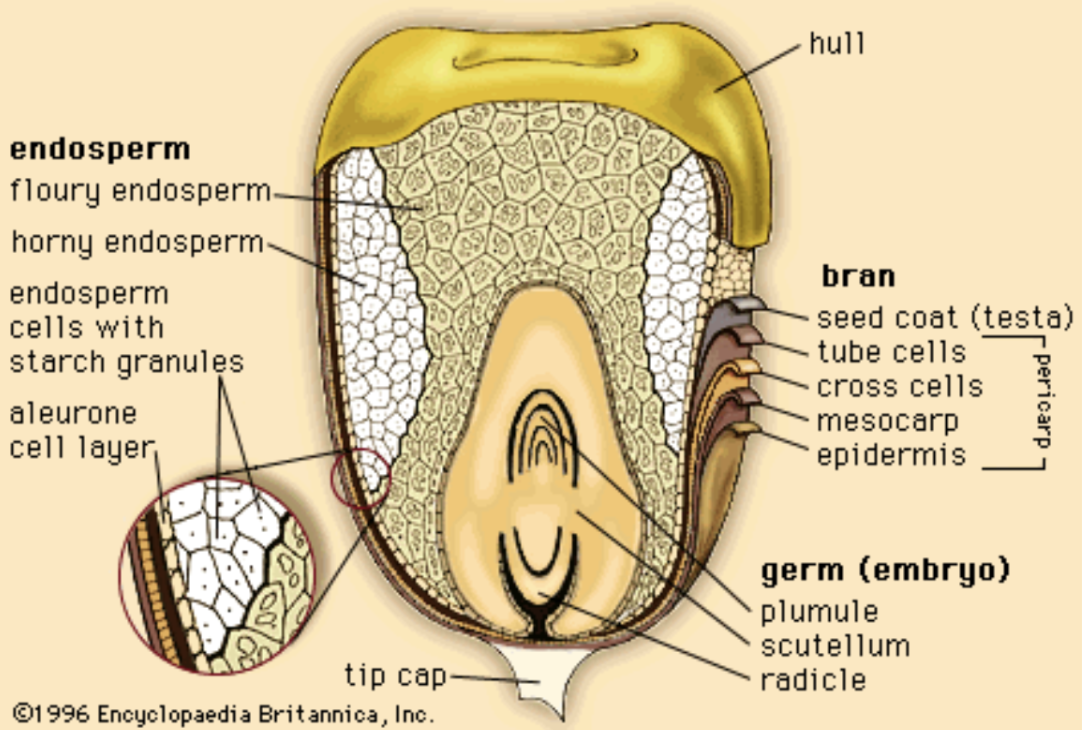
\includegraphics[width=\linewidth]{figura1.png}
    \captionof{figure}{Grano de maíz (Kent-Jones y Singh, 2024)}
\end{Figure}

El endospermo almacena las reservas de proteínas y almidón de la semilla y es consumido por el embrión durante la maduración de la misma \cite{13}. Aunque la composición química de los endospermos varía entre especies, normalmente contienen mioinositol, sorbitol, auxinas, citoquininas, y compuestos nitrogenados \cite{6}. Los medios de cultivo con frecuencia son suplementados con sustancias que ayudan al desarrollo del embrión. Las auxinas, por ejemplo (IAA, NAA, 2,4-D, o IBA) se adicionan para la división e iniciación de raíces. Sin embargo, altas concentraciones de estas sustancias pueden llegar a suprimir la morfogénesis. La auxina 2,4-D es comúnmente empleada para la inducción de callo, mientras que las auxinas IAA, IBA y NAA son usadas para la inducción de raíces. \cite{4} 

Por último, el momento propicio para llevar a cabo el rescate también dependerá de la etapa promedio en la que ocurre el aborto del embrión en la planta. Además, se debe considerar que, cuanto más tiempo se pueda desarrollar el embrión en la planta (estado de madurez más allá de la etapa globular), más fácil será aislarlo y cultivarlo exitosamente. \cite{2}

\textbf{
\section{Materiales}
}

\textit{2.1.- Material biológico}

Granos de elote\textit{ (Zea mays) }comercial de HEB.

\textit{2.2.- Reactivos}

Agua estéril, solución de hipoclorito al 2\%, solución de EtOH al 70\%, EtOH al 96\%, una caja Petri con medio MS a carga completa con ácido indol-3-acético (IAA) (0.1mg/L),  una caja Petri con medio MS a carga completa con ácido naftalenacético (NAA) (0.1mg/L), dos cajas Petri con medio MS a carga completa con acido indol butirico (IBA) (0.1mg/L) y una caja Petri con medio MS a carga completa.

\textit{2.3.- Equipos}

Campana de flujo laminar de nivel 1 (LABCONCO)

\section{Metodología y Resultados}

\textit{\textbf{3.1 }}\textit{Etapa preanalítica}

La campana se limpió con etanol al 70\% y se introdujo el material de trabajo previamente rociado con la solución de etanol al 70\%.

\textit{\textbf{3.2 }}\textit{Etapa analítica}

Se preparó el explante seleccionando, una mazorca fresca, quitando las hojas y brácteas, removiendo los granos individualmente evitando dañar el pericardio. Se seleccionaron 35 granos aleatoriamente, los cuales fueron lavados con agua corriente y jabón por 3 min. Se retiró el agua del vaso y se introdujo en la campana.

\textit{\textbf{3.2.1 }}\textit{Técnica aséptica}

La primera etapa de desinfección de los granos fue el remojo con etanol al 70\% por 1 minuto, posteriormente se decantó el etanol. Se continuó con la desinfección sumergiendo los granos en la solución de hipoclorito de sodio al 2\% por 15 minutos, y se decantó el hipoclorito. Por último se realizó un lavado con agua destilada esterilizada y se decantó.

\textit{\textbf{3.2.2 }}\textit{Rescate de embriones }

Se sostuvo el grano con las pinzas, sobre una caja Petri esteril y se realizaron cortes longitudinales en la superficie frontal del grano con el bisturí (figura 2). Se insertó la parte plana del bisturí y se empujó hasta que se observó la salida forzada del embrión. El proceso se repitió con 25 granos previamente desinfectados.

\begin{Figure}
    \centering
    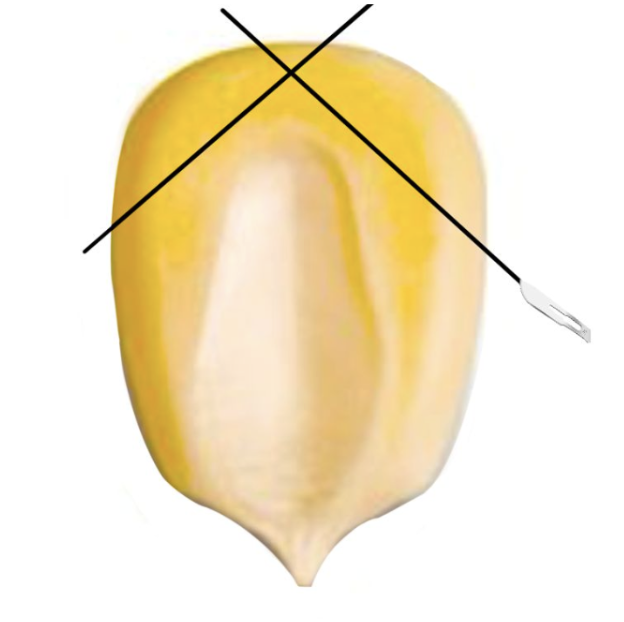
\includegraphics[width=0.7\linewidth]{figura2.png}
    \captionof{figure} {Rescate de embrión de grano de maíz}
\end{Figure}

\textit{\textbf{3.2.3 }}\textit{Siembra del explante }

Se colocaron 5 embriones por cada caja Petri, colocando 4 de los embriones en las esquinas  de la caja y uno en el centro (figura 3). Posteriormente se sellaron las cajas Petri con papel parafilm.

\begin{Figure}
    \centering
    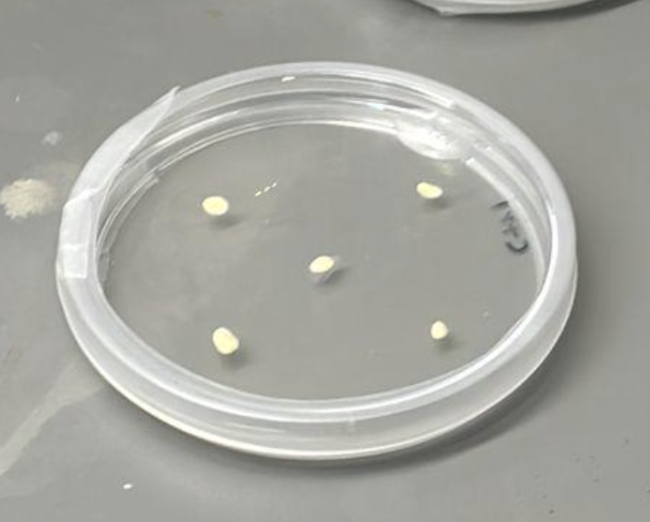
\includegraphics[width=0.7\linewidth]{figura3.png}
    \captionof{figure}{\textit{Caja Petri con los embriones de maíz}}
\end{Figure}

\textit{\textbf{3.3}}\textit{ Etapa postanalítica}

Las cajas Petri de los tratamientos, control, IBA, INA, IAA, se colocaron en las condiciones de fotoperiodo 12h Luz - 12h Oscuridad con y a una temperatura de 27ºC. La caja Petri restante, con el tratamiento de IBA se colocó en condiciones de fotoperiodo 24h Oscuridad, a una temperatura 30ºC. Se tomaron mediciones por 10 días hábiles siendo el 19 de agosto del 2024 la fecha inicial y el 30 de agosto del 2024 la fecha final. \cite{16} 

\textbf{
\section{Resultados}
}

\textit{\textbf{4.1.}}\textit{ Resultados cualitativos}

\textit{\textbf{4.1.1}}\textit{ Fotoperiodo 12 h Luz}

En la figura 4 (a) se puede observar el crecimiento de la plántula control y presencia de contaminantes. En los embriones cultivados en medio MS adicionado con IAA (figura 4, b) se observa una plántula con crecimiento libre de contaminación, en donde se pueden observar raíces, tallos y hojas; de igual forma, para el cultivo con medio MS suplementado con IBA  figura 4 (c), donde se observa el crecimiento de 3 semillas sin contaminación. Finalmente los embriones tratados con NAA (figura 4, d) se observa igualmente un crecimiento libre de contaminantes, sin embargo, a diferencia de los demás se observa mayor cantidad de raíces y menor cantidad de hojas. Los resultados de crecimiento son reportados después de 10 días hábiles de crecimiento.

\begin{Figure}
    \centering
    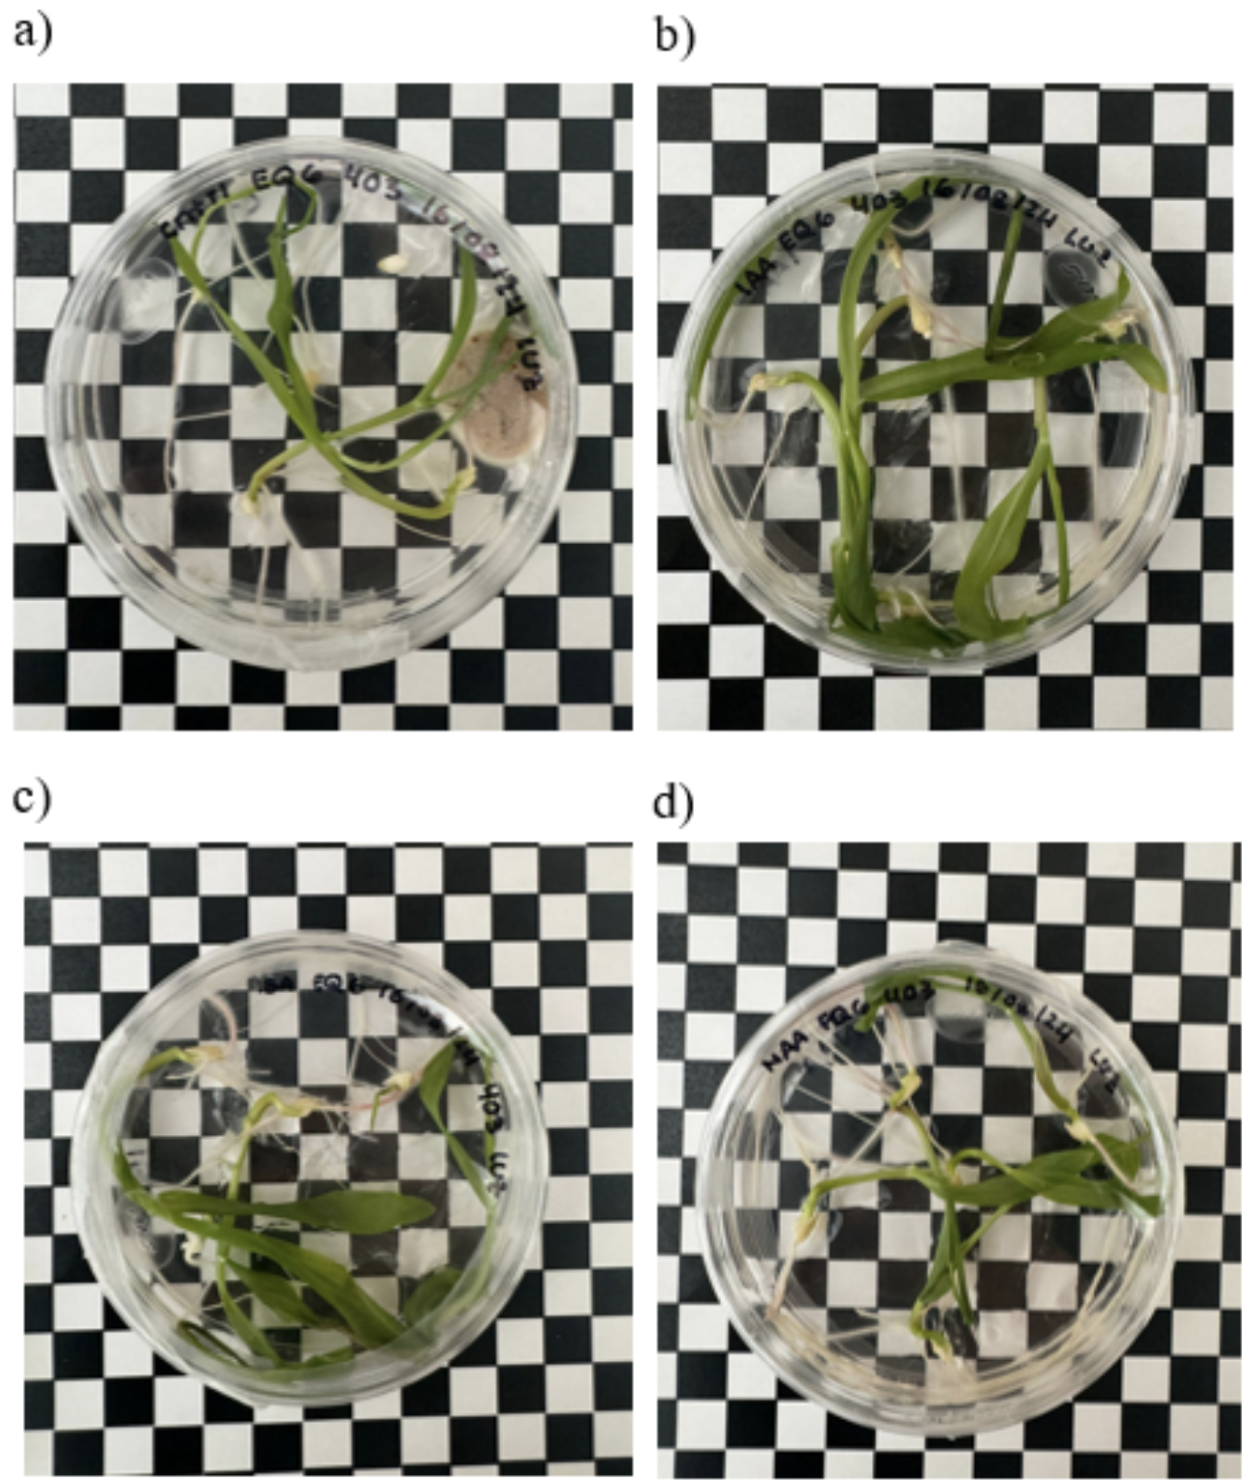
\includegraphics[width=0.7\linewidth]{figura4.png}
    \captionof{figure}{Décimo día de germinación de cultivo de embriones de maíz en fotoperiodo 12 h Luz 12h Oscuridad. a) Control. b) Medio MS suplementado con IAA c)Medio MS suplementado con IBA d)Medio MS suplementado con NAA}
\end{Figure}

\textit{\textbf{4.1.2}}\textit{ Fotoperiodo 24h  Oscuridad}

\begin{Figure}
    \centering
    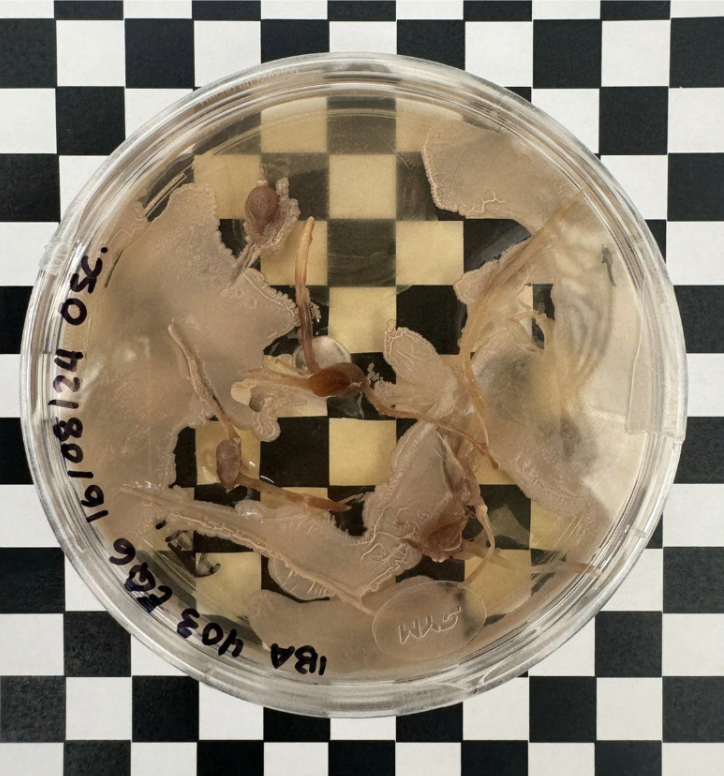
\includegraphics[width=0.7\linewidth]{figura5.png}
    \captionof{figure}{Décimo día de germinación. Embriones de maíz cultivados en medio MS suplementado con IBA en fotoperiodo 24h de oscuridad.}
\end{Figure}

En la figura 5 se puede observar el crecimiento de tallo prácticamente nulo, y una alta presencia de contaminantes. Los embriones lograron crecer raíces sin embargo no se observan tallos ni hojas. Además el medio se tornó a una tonalidad turbia. 

\textit{\textbf{4.2.}}\textit{ Resultados cuantitativos}

\textit{\textbf{4.2.1 }}\textit{Germinación de embriones}

Se realizaron cuatro factores (fotoperiodo 12h Luz-12h Oscuridad, fotoperiodo 24h oscuridad,  cantidad de raíces, cantidad de tallos y cantidad de callos) cada uno con cuatro niveles (control, medio MS suplementado con NAA, medio MS suplementado con IBA , y medio MS suplementado con IAA), y tres repeticiones por cada nivel. Los datos que se presentan son promedio ± desviación estándar. Para cada factor, se realizó un análisis de varianza, y las medias se compararon por método de Tukey con una confianza al 95\%. Todos los análisis estadísticos se llevaron a cabo en Minitab  21.4.2. Los valores de p menores a 0.05 fueron considerados estadísticamente significativos. 


\begin{table*}[ht]
\centering
\begin{tabularx}{\textwidth}{ | X | X | X | X | }
\toprule
\rowcolor[HTML]{EFEFEF} 
Auxina  & Cantidad de raíces & Cantidad de tallos & Cantidad de callos \\ \midrule
Control & 17.0±15.62A        & 5.67±2.08A         & 0                  \\ \midrule
NAA     & 16.67±2.08A        & 6.33±1.15A         & 0                  \\ \midrule
IBA     & 18.67±10.97A       & 6.67±2.08A         & 0                  \\ \midrule
IAA     & 10.33±9.24A        & 6.0± 1.0A          & 0                  \\ \bottomrule
\end{tabularx}
\caption{Germinación en fotoperiodo 12h Luz-12h Oscuridad}
\end{table*}

    
Los resultados obtenidos para la cantidad de raíces en embriones en fotoperiodo 12h luz- 12h oscuridad (Tabla 1) no fueron estadísticamente significativos, con un valor de p igual a 0.787 para los resultados de semillas germinadas, y 0.892 para los resultados de cantidad de tallos (Tabla 1), con una desviación estándar agrupada de 10.65  y 1.65, respectivamente. 


\begin{table*}[ht]
\centering
\begin{tabularx}{\textwidth}{ | X | X | X | X | }
\toprule
\rowcolor[HTML]{EFEFEF} 
Auxina  & Cantidad de raíces & Cantidad de tallos & Cantidad de callos \\ \midrule
Control & 8.33±1.528B        & 3.67±0.577A        & 0                  \\ \midrule
NAA     & 18.33± 5.69A       & 4.667±0.577A       & 0                  \\ \midrule
IBA     & 11.0± 2.65AB       & 3.0±2.65A          & 0                  \\ \midrule
IAA     & 7.67± 2.89B        & 4.667±0.577A       & 0                  \\ \bottomrule
\end{tabularx}
\caption{Germinación en fotoperiodo 24h Oscuridad}
\end{table*}


Los resultados obtenidos para la cantidad de raíces en los embriones en fotoperiodo 24h oscuridad (Tabla 2) sí fueron estadísticamente significativos, con un valor de p igual a 0.022, mientras que para la cantidad de tallos (Tabla 2) no lo fueron, con un valor de p igual a 0.441; con una desviación estándar agrupada de 3.533 y 1.41, respectivamente. 

\section{Análisis de resultados}

En la germinación de semillas del tratamiento control se observó el crecimiento después de 72 h posteriores a la germinación donde se desarrollaron los brotes del 80\% de las semillas en el tratamiento.  Mismo comportamiento se reportó por \cite{12} donde los embriones comenzaron a desarrollar brotes y raíces dentro de las 24 - 36 h posteriores a la germinación en la regeneración de plantas en medio MS sin fitorreguladores, con una eficiencia de germinación de 67\%. 

La germinación de embriones bajo el fotoperiodo de 12 horas de luz y 12 horas de oscuridad mostró un mayor crecimiento de raíces y tallos, en comparación con el fotoperiodo de 24 h de oscuridad, con excepción de las plántulas en el tratamiento con NAA en oscuridad , donde se observó una mayor cantidad de raíces (18.33± 5.69\textsubscript{A}). A diferencia de esto, en otras especies de plantas se ha observado que los tratamientos en condición de oscuridad en el rescate de embriones de banano  fueron superiores a los tratados en condiciones de luz/oscuridad tanto para la tasa de crecimiento como la longitud de los brotes de las plántulas de banano germinadas \cite{3}. 

La estadística de los resultados demostró que los embriones de maíz no requieren de fitorreguladores para llevar a cabo su morfogénesis, dado que no se encontraron diferencias significativas entre las tres auxinas probadas y el control. Sin embargo, \cite{9} menciona que el elote es un cultivo demandante y necesita de una aplicación balanceada de nutrientes y demuestra que el uso de diferentes concentraciones de NAA y nitrógeno sí presentan significancia en la altura y la tasa de crecimiento del elote. \cite{18} 

También se ha visto que el  uso de auxinas en otras especies de plantas, donde se presenta un alto grado de significancia, por ejemplo, en el rescate de embriones de banano \cite{7}, donde, en conjunto con medios suplementados con auxinas IAA y BA resultaron en una mayor regeneración de plántulas. 

En el estudio realizado por Godoy et al., 2006 se generaron callos embriogénicos con una concentración de 1,2 y 5 mg/L de de auxina ácido 2,4- diclorofenoxiacético (2,4-D) , y se observó el crecimiento de radícula y meristemos apical en el medio sin fitorreguladores pero suplementado con nutrientes \cite{20}.  En comparación con lo realizado se infiere que la ausencia de formación de callo se debe a la concentración de auxinas empleada (0.1mg/L), siendo la reportada, entre 10-50 veces mayor que la utilizada en este estudio. \cite{19}

Asimismo se observó contaminación en 2 de los 5 medios tratados, y, de acuerdo con Cassells, 2012, la presencia de contaminantes en el medio se originan por microorganismos presentes en  los explantes sembrados o por la manipulación y/o almacenaje incorrecto y el desarrollo de estos agentes contaminantes en nuestro cultivo se debe a la alta concentración de nutrientes presentes en el medio MS. \cite{1}   

\section{Conclusiones}

El rescate de embriones es una técnica ampliamente utilizada en el cultivo vegetal \textit{in vitro}, ya que permite desarrollar y preservar especies vegetales mejoradas, como consecuencia del entrecruzamiento genético. La selección del tipo de medio, la concentración de fitorreguladores y las condiciones de los tratamientos dependen del tipo de especie de la planta. Además, es importante definir qué tipo de crecimiento se busca generar con el fin de seleccionar la concentración de fitoreguladores adecuada para su tratamiento. En contraste con lo reportado en literatura,  los resultados estadísticos de esta práctica indican inconsistencias \cite{17}, las cuales se deben a las concentraciones bajas de auxinas utilizadas y a la falta de monitoreo de la procedencia de la planta manejada, es decir no se conocía su edad y condiciones de crecimiento. 

A la par,  se presentó contaminación en varios de los cultivos, generando interferencias en el comportamiento y desarrollo de la planta, determinando que los resultados de este ensayo no fueron óptimos.


\section{Perspectivas}
Se sugiere mejorar las técnicas de desinfección y esterilización del laboratorio con el fin de poder monitorear el crecimiento sin la presencia de patógenos, ya que imposibilitan el desarrollo óptimo de la planta y perjudican los datos estadísticos recabados. Por otro lado, si se planea producir callo embrionario se sugiere aumentar la concentración de auxinas en el medio. Siguiendo la práctica y tomando en cuenta las consideraciones establecidas se obtendrán con éxito resultados que permitan realizar un análisis estadístico óptimo. 


\bibliography{referenciasProyecto}
 

\end{multicols}
\end{document}
